%% ----------------------------------------------------------------
%% Management.tex
%% ---------------------------------------------------------------- 

\chapter{Project Management} \label{Chapter:Project Management}

The software is a kind of intangible product. Most software products are tailored to conform to specific requirements. More importantly, the underlying technology frequently changes and progress rapidly, Therefore, the development procedure of a product may not be suitable for another. All of these businesses and constraints result in the risks in software development, so it is crucial to managing the software project effectively. 


\section{Project Constraints}



As shown in Figure 3.1, software projects normally have three constraints, schedule, budget and scope. It is an essential part of software developers to develop high-quality products, to keep costs within budget limits, and to deliver products on time. There are several factors, including internal and external, which may affect the triple constraint triangle. The three constraints are interdependent: None of them can be altered without affecting one or both of the others. Therefore, the software project management is crucial to incorporate user requirements along with time constraints and budget limits.


\begin{figure}[H]
  \centering
  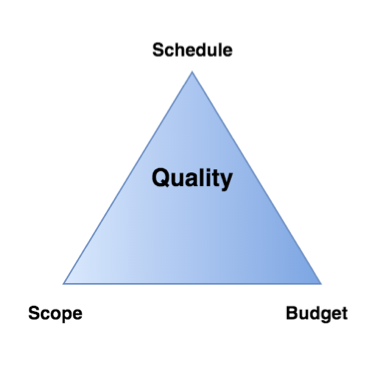
\includegraphics[width=6cm]{./img/Picture1}
  \caption{Triple Constraint Triangle}
  \label{Figure:figex}
\end{figure}


According to the triple constraint triangle above, the constraints that may delay the progress of this project are listed as follows:

\textbf{Schedule}: The duration of the project is only three months, so it is necessary to have a time management plan to ensure the project can be accomplished on time.

\textbf{Budget}: There is no budget available for this project. As such, it may restrict the access to some open datasets, because some open APIs require users to pay for more operations.

\textbf{Scope}: Due to the limitations of time and budget, the scope of this project is to meet basic requirements to complete this project on time and within budget limits.


\section{Project Methodology}

The Iterative and Incremental development model will be employed for the development of this project. In this model, the project is designed, implemented and tested incrementally until the product is finished. Also, it involves both development and maintenance. The project is defined as completed when it satisfies all of its requirements. Following this model, this project will be developed step by step. 


Figure 3.2 illustrates that the development lifecycle of this model is divided into three stages. The first stage is initial planning, which compromises the problem identification, system and requirements analysis, and system design. Then, the second stage is decomposed into some build cycles, which is designed and built separately. Each incremental build consists of the detailed design, implementation, testing and evaluation \cite{4_houston_2011}. Each build is delivered to the clients until the complete product is delivered. In this way, developers can obtain regular feedback throughout the whole lifecycle and avoid a long development time. Once all requirements are met, the final stage is to deploy the system.

\begin{figure}[H]
  \centering
  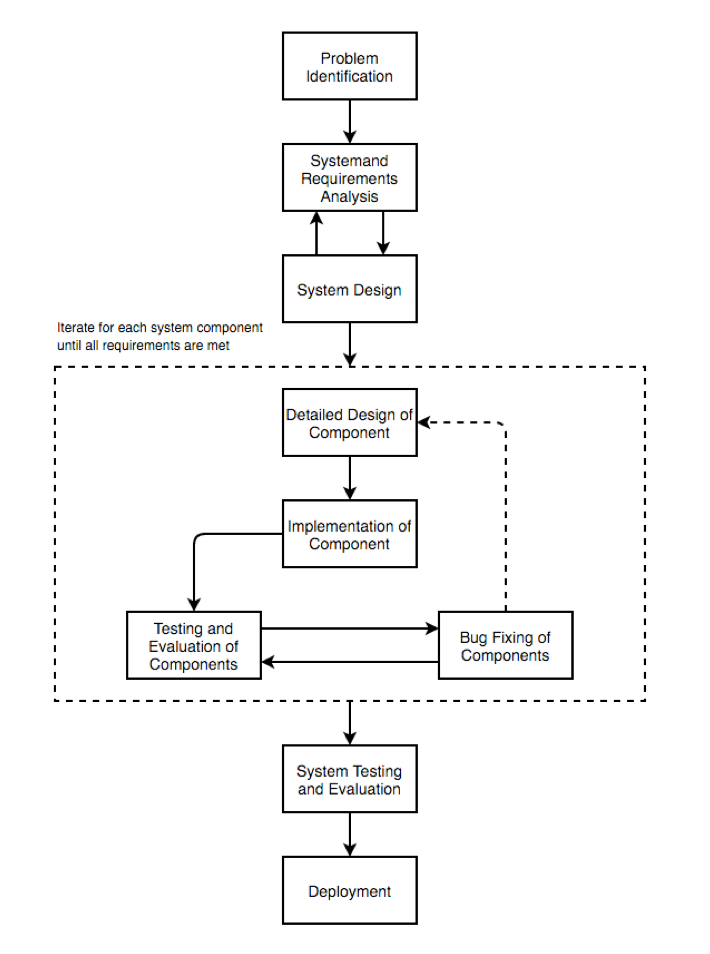
\includegraphics[width=12cm]{./img/Picture2}
  \caption{The Iterative and Incremental Development Model}
  \label{Figure:figex}
\end{figure}


\section{Time Management}

As mentioned above, the schedule is one of three constraints that hold the key to high-quality products. Hence, it is important to have a time management to ensure this project can be completed on time and achieve all user requirements.  Figure 3.3 is a Gantt chart, which includes all tasks and timings for this project. It can help distribute estimated effort to specific tasks across the duration of this project.

\begin{figure}[H]
  \centering
  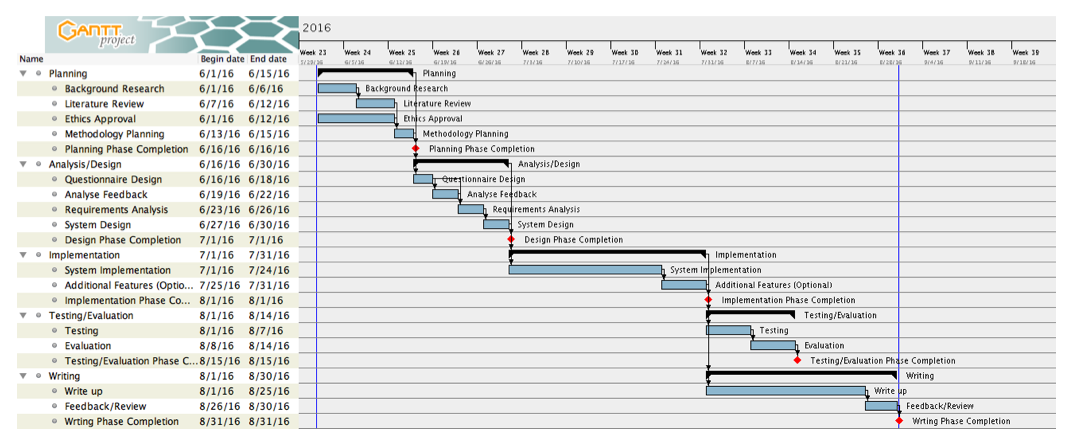
\includegraphics[width=15cm]{./img/Picture3}
  \caption{Gantt Chart}
  \label{Figure:figex}
\end{figure}

\textbf{Phase 1: Planning (2 Weeks)}

The first phase is project planning. In this phase, the background research will be conducted, which will focus on the general topic, open data, data visualisation and the relevant implementation technologies or tools. Then, the literature review about the application of open data and data visualisation in educational choices will be conducted to identify research questions, project aims and objectives. Afterwards, application documents will be submitted to ERGO committee to apply for the ethical approval. Finally, the methodology and schedule of this project will be planned.

\textbf{Phase 2: Analysis/Design (2 Weeks)}

The second phase is about requirements analysis and system design. Firstly, a questionnaire will be designed to identify factors influencing international students’ decision-making process for higher education in the UK. Based on the results of the survey, user requirements will be analysed and identified. Meanwhile, it is necessary to search for or collect relevant open datasets that reflect those factors. Afterwards, the detailed system requirements including functional and non-functional requirements will be derived from requirements analysis.

\textbf{Phase 3: Implementation (4 Weeks)}

The implementation phase is divided into two parts. The first part is system implementation, which is implemented using the technologies or tools analysed in Phase 1 and adhere to the proposed system design. The second part, which is optional is to add additional features according to users’ feedback during each incremental build. Also, this phase will overlap with phase 2 and phase 4, as all system requirements will be implemented and tested iteratively and incrementally in the development lifecycle.

\textbf{Phase 4: System Testing/ Evaluation (2 Weeks)}

In this phase, system testing, including black box and white box tests will be carried out to test the functional requirements and validate the non-functional requirements. Afterwards, the resulting web application and the whole process will be evaluated.

\textbf{Phase 5: Dissertation Writing (4 Weeks)}

This final phase is to write up the dissertation and modify it based on supervisor’s feedback. This phase and phase 4 will start at the same time as the implementation phase is completed.



\section{Risk Analysis and Management}

Risk analysis and management process is a significant step in preparation for potential risks that can occur within any software project. It can ensure any software project can be accomplished smoothly and successfully. Therefore, it is important to identify and analyse potential risks before they occur, and find appropriate measures to avoid and manage them \cite{boehm1991software}.


\subsection{Risk Identification}

The first step is to identify potential risks that can affect the success of the project. Table 3.1 provides an overview of all identified risks that can occur in this project based on Boehm's \cite{boehm1991software} prioritized top-ten list of software risks items.


\begin{table}[H]
\centering
\caption{Risk Identification}
\label{my-label}
\begin{tabular}{|p{3cm}|p{5cm}|p{5cm}|}
\hline
\textbf{Category}              & \textbf{Risk Item}                       & \textbf{Description}                                                                      \\ \hline
Personnel management risks     & Personnel shortfalls                     & Illness and other personal issues delay the completion of the project                     \\ \hline
Schedule and timing            & Unrealistic schedules and budgets        & Project cannot complete on time due to incorrectly estimated development time and budget  \\ \hline
System and functionality       & Developing the wrong software functions  & Development of software functions cannot meet users’ requirements                         \\ \cline{2-3} 
                               & Developing the wrong user interface      & Inadequate design of user interface and difficulties in usability and accessibility       \\ \hline
Requirement management         & Gold plating                             & Development of  unnecessary functions or features that not asked for by users             \\ \cline{2-3} 
                               & Continuing stream of requirement changes & Uncontrolled and unpredictable changes in system requirements or design                   \\ \hline
Resource usage and performance & Real-time performance shortfalls         & Poor system performance compromise the functionality or lead system failure               \\ \cline{2-3} 
                               & Straining computer-science capabilities  & Inability to implement the system due to lack of relevant technical solutions or datasets \\ \hline
\end{tabular}
\end{table}


\subsection{Risk Analysis}


The second step to evaluate the level and the severity of each risk in combination with the occurrence probability. Sommerville \cite{5_sommerville_2011} suggested a standard to describe the seriousness of the risks as follow:

1.	Probability: The probability of the risk might be assessed as very low (10\%), low (10-25\%), moderate (25-50\%), high (50-70\%), or very high (75\%).

2.	Effect: The effects of the risk might be assessed as catastrophic (threaten the survival of the project), serious (would cause major delays), tolerable (delays are within allowed contingency), or insignificant.

Table 3.2 displays the analysis of potential risks in this project, including their effects, occurrence probabilities and risk levels. 

\begin{table}[H]
\centering
\caption{Risk Analysis}
\label{my-label}
\begin{tabular}{|p{4cm}|p{3cm}|p{3cm}|p{3cm}|}
\hline
\textbf{Risk Item}                       & \textbf{Probability} & \textbf{Effect} & \textbf{Risk Level} \\ \hline
Personnel shortfalls                     & 10\%                 & Tolerable       & Low                 \\ \hline
Unrealistic schedules and budgets        & 70\%                 & Serious         & High                \\ \hline
Developing the wrong software functions  & 50\%                 & Catastrophic    & Moderate            \\ \hline
Developing the bad user interface        & 50\%                 & Catastrophic    & Moderate            \\ \hline
Gold plating                             & 40\%                 & Tolerable       & Moderate            \\ \hline
Continuing stream of requirement changes & 20\%                 & Tolerable       & Low                 \\ \hline
Real-time performance shortfalls         & 60\%                 & Serious         & High                \\ \hline
Straining computer-science capabilities  & 70\%                 & Serious         & High                \\ \hline
\end{tabular}
\end{table}

\subsection{Risk Management}

The final step to develops strategies to manage these potential risks. According to Sommerville \cite{5_sommerville_2011}, catastrophic risks should always be considered, as should all serious risks that have more than a moderate probability of occurrence. Therefore, mitigation strategies of identified risks are suggested in Table 3.3 to ensure that all risks are limited to minimum danger for the project.

\begin{table}[H]
\centering
\caption{Risk Management}
\label{my-label}
\begin{tabular}{|p{4cm}|p{10cm}|}
\hline
\textbf{Risk Item}                       & \textbf{Mitigation Strategy}                                                                               \\ \hline
Personnel shortfalls                     & 1. Try to work ahead of the schedule to have a time buffer                                             \\
                                         & 2. Work on weekends to catch up the delay                                                              \\ \hline
Unrealistic schedules and budgets        & 1. Divide the project into small tasks and establish specific phased targets                           \\
                                         & 2. Arrange weekly meeting with supervisor to discuss tasks, difficulties and challenges                \\ \hline
Developing the wrong software functions  & 1. Design the questionnaire carefully and scientifically to cover all requirements that users may need \\
                                         & 2. Analyse and design the requirements thoroughly                                                      \\
                                         & 3. Arrange weekly meeting with supervisor to discuss the requirements                                  \\ \hline
Developing the wrong user interface      & 1. Arrange weekly meeting with supervisor to discuss the interface and design                          \\
                                         & 2. Invite friends or peers to experience the interface and design, and ask for advice or suggestions   \\ \hline
Gold plating                             & 1. Stick strictly to the user requirements                                                             \\
                                         & 2. Focus on functionality first, then on the design                                                    \\ \hline
Continuing stream of requirement changes & 1. Design the questionnaire carefully and scientifically to cover all requirements that users may need \\
                                         & 2. Analyse and design the requirements thoroughly to avoid later changes                               \\ \hline
Real-time performance shortfalls         & 1. Choose appropriate technologies or tools to implement this project                                  \\
                                         & 2. Test and evaluate regularly to solve bugs and optimize the code                                     \\ \hline
Straining computer-science capabilities  & 1. Choose suitable technologies or tools and available datasets to implement this project              \\
                                         & 2. Ask friends for help or ask questions on forums, like stackoverflow.com                             \\ \hline
\end{tabular}
\end{table}


\section{Summary}
This chapter outlines information on project management. The triple constraint triangle, which consists of schedule, budget and scope are used to identify the project constraints. Then, the project methodology, iterative and incremental development model is introduced to explain how this project is developed. Afterwards, a Gantt chart is used to explain how the tasks and timings are managed among the phases of this project. Finally, potential risks, like personnel shortfalls are identified, and mitigation strategies of these risks are outlined to ensure the success of this project.

